\documentclass[oneside,final,12pt, a4paper]{extreport}
\linespread{1.3}
\usepackage[utf8]{inputenc}
\usepackage[russian]{babel}

\usepackage{hyperref} % for clickable links

\usepackage{titlesec}
\setcounter{secnumdepth}{4}
\setcounter{tocdepth}{4}
\titleformat{\paragraph} % for more deeper subsections
{\normalfont\normalsize\bfseries}{\theparagraph}{1em}{}
\titlespacing*{\paragraph}
{0pt}{3.25ex plus 1ex minus .2ex}{1.5ex plus .2ex}

\usepackage{amsmath} % for math formula
\usepackage{amssymb} % for math formula

\usepackage[]{graphicx}
\usepackage{graphbox} % align in images
\usepackage{wasysym}
\graphicspath{{images/}} % path to images

\newcommand{\etal}{\textit{et al}. } % for citation

\newcommand{\sect}[1]{%
  \newpage%
  \section*{#1}%
  \addcontentsline{toc}{section}{#1}}
\newcommand\subsect[1]{%
  \subsection*{#1}%
  \addcontentsline{toc}{subsection}{#1}}

\usepackage{subcaption}
\usepackage{mwe}
\usepackage{titlesec}
\usepackage[left=3cm,right=1.5cm,top=2cm,bottom=2cm]{geometry}
\usepackage{indentfirst}
\sloppy


\titleformat{\chapter}
{\normalfont\LARGE\bfseries}{\thechapter ~~}{0pt}{\LARGE}
\titlespacing*{\chapter} {0pt}{0pt}{20pt}

\begin{document}
\title{Дипломная работа}
\author{Щербаков Александр Станиславович}
\date{2019}
\begin{titlepage}
  \begin{center}
    \begin{figure}[h!]
      \center    
      
\includegraphics{title/msu.jpg}
    \end{figure}
    Московский государственный университет имени М.В. Ломоносова\\
    Факультет вычислительной математики и кибернетики\\
    Кафедра интеллектуальных информационных технологий\\
    \vspace{2.3cm}
    {\LARGE Щербаков Александр Станиславович \\
    \vspace{1.24cm}
    \textbf{Динамическая и иерархическая излучательность\\}
    \vspace{2.2cm}
    МАГИСТЕРСКАЯ ДИССЕРТАЦИЯ \\
    }
    \vspace{3.4cm}
    \hfill { \bf Научный руководитель:\\}
    \hfill к.ф-м.н., научный сотрудник\\
    \hfill В. Ф. Фролов \\
    \vfill Москва, 2019
  \end{center}
\end{titlepage}
\pagebreak

%--------------------------------------------------------------------------------

\tableofcontents

\sect{Аннотация}

В данной работе предлагается новый подход к вычислению глобального освещения для больших 3D-сцен. Выделяют два вида освещения: первичное - прямое освещени от источника, и вторичное - свет, отраженный поверхностями. Основную сложность представляет вычисление именно вторичного освещения, так как значение переотраженного света выражается в виде многомерного интеграла. К современным приложениям, поддерживающим визуализацию реалистичных 3D-сцен, предъявляются жесткие требования на время работы алгоритма. При этом размеры и сложность сцен постоянно увеличиваются.
В ходе работы была разработана модификация метода излучательности, которая позволяет сосредоточить основные ресурсы компьютера на вычислении освещения для 3D-объектов, вносящих наибольший вклад в изображение. Новый метод способен производить вычисление глобального освещения за время, не превосходящее 2 мс в том числе на видеокартах для ноутбуков, с сохранением приемлемого качества изображения.

\sect{Введение}

Задача вычисления глобального освещения является одной из основных задач в приложениях реального времени, связанных с 3D-визуализацией. Свет падающий на поверхности объектов, складывается из лучей, выпущенных источниками света (первичное освещение), и лучей, отраженных поверхностями (вторичное освещение) (Рис. \ref{fig:Lighting}). При этом задача вычисления вторичного освещения является более сложной, чем вычисление первичного. Это связано с необходимостью вычисления многомерного интеграла для каждого отражения \cite{RT_rendering}. Для данной компоненты освещения используются различные приближения и численные методы, так как аналитическое решение не представляется возможным, особенно в приложениях реального времени.

\begin{figure}[htb]
  \begin{center}
  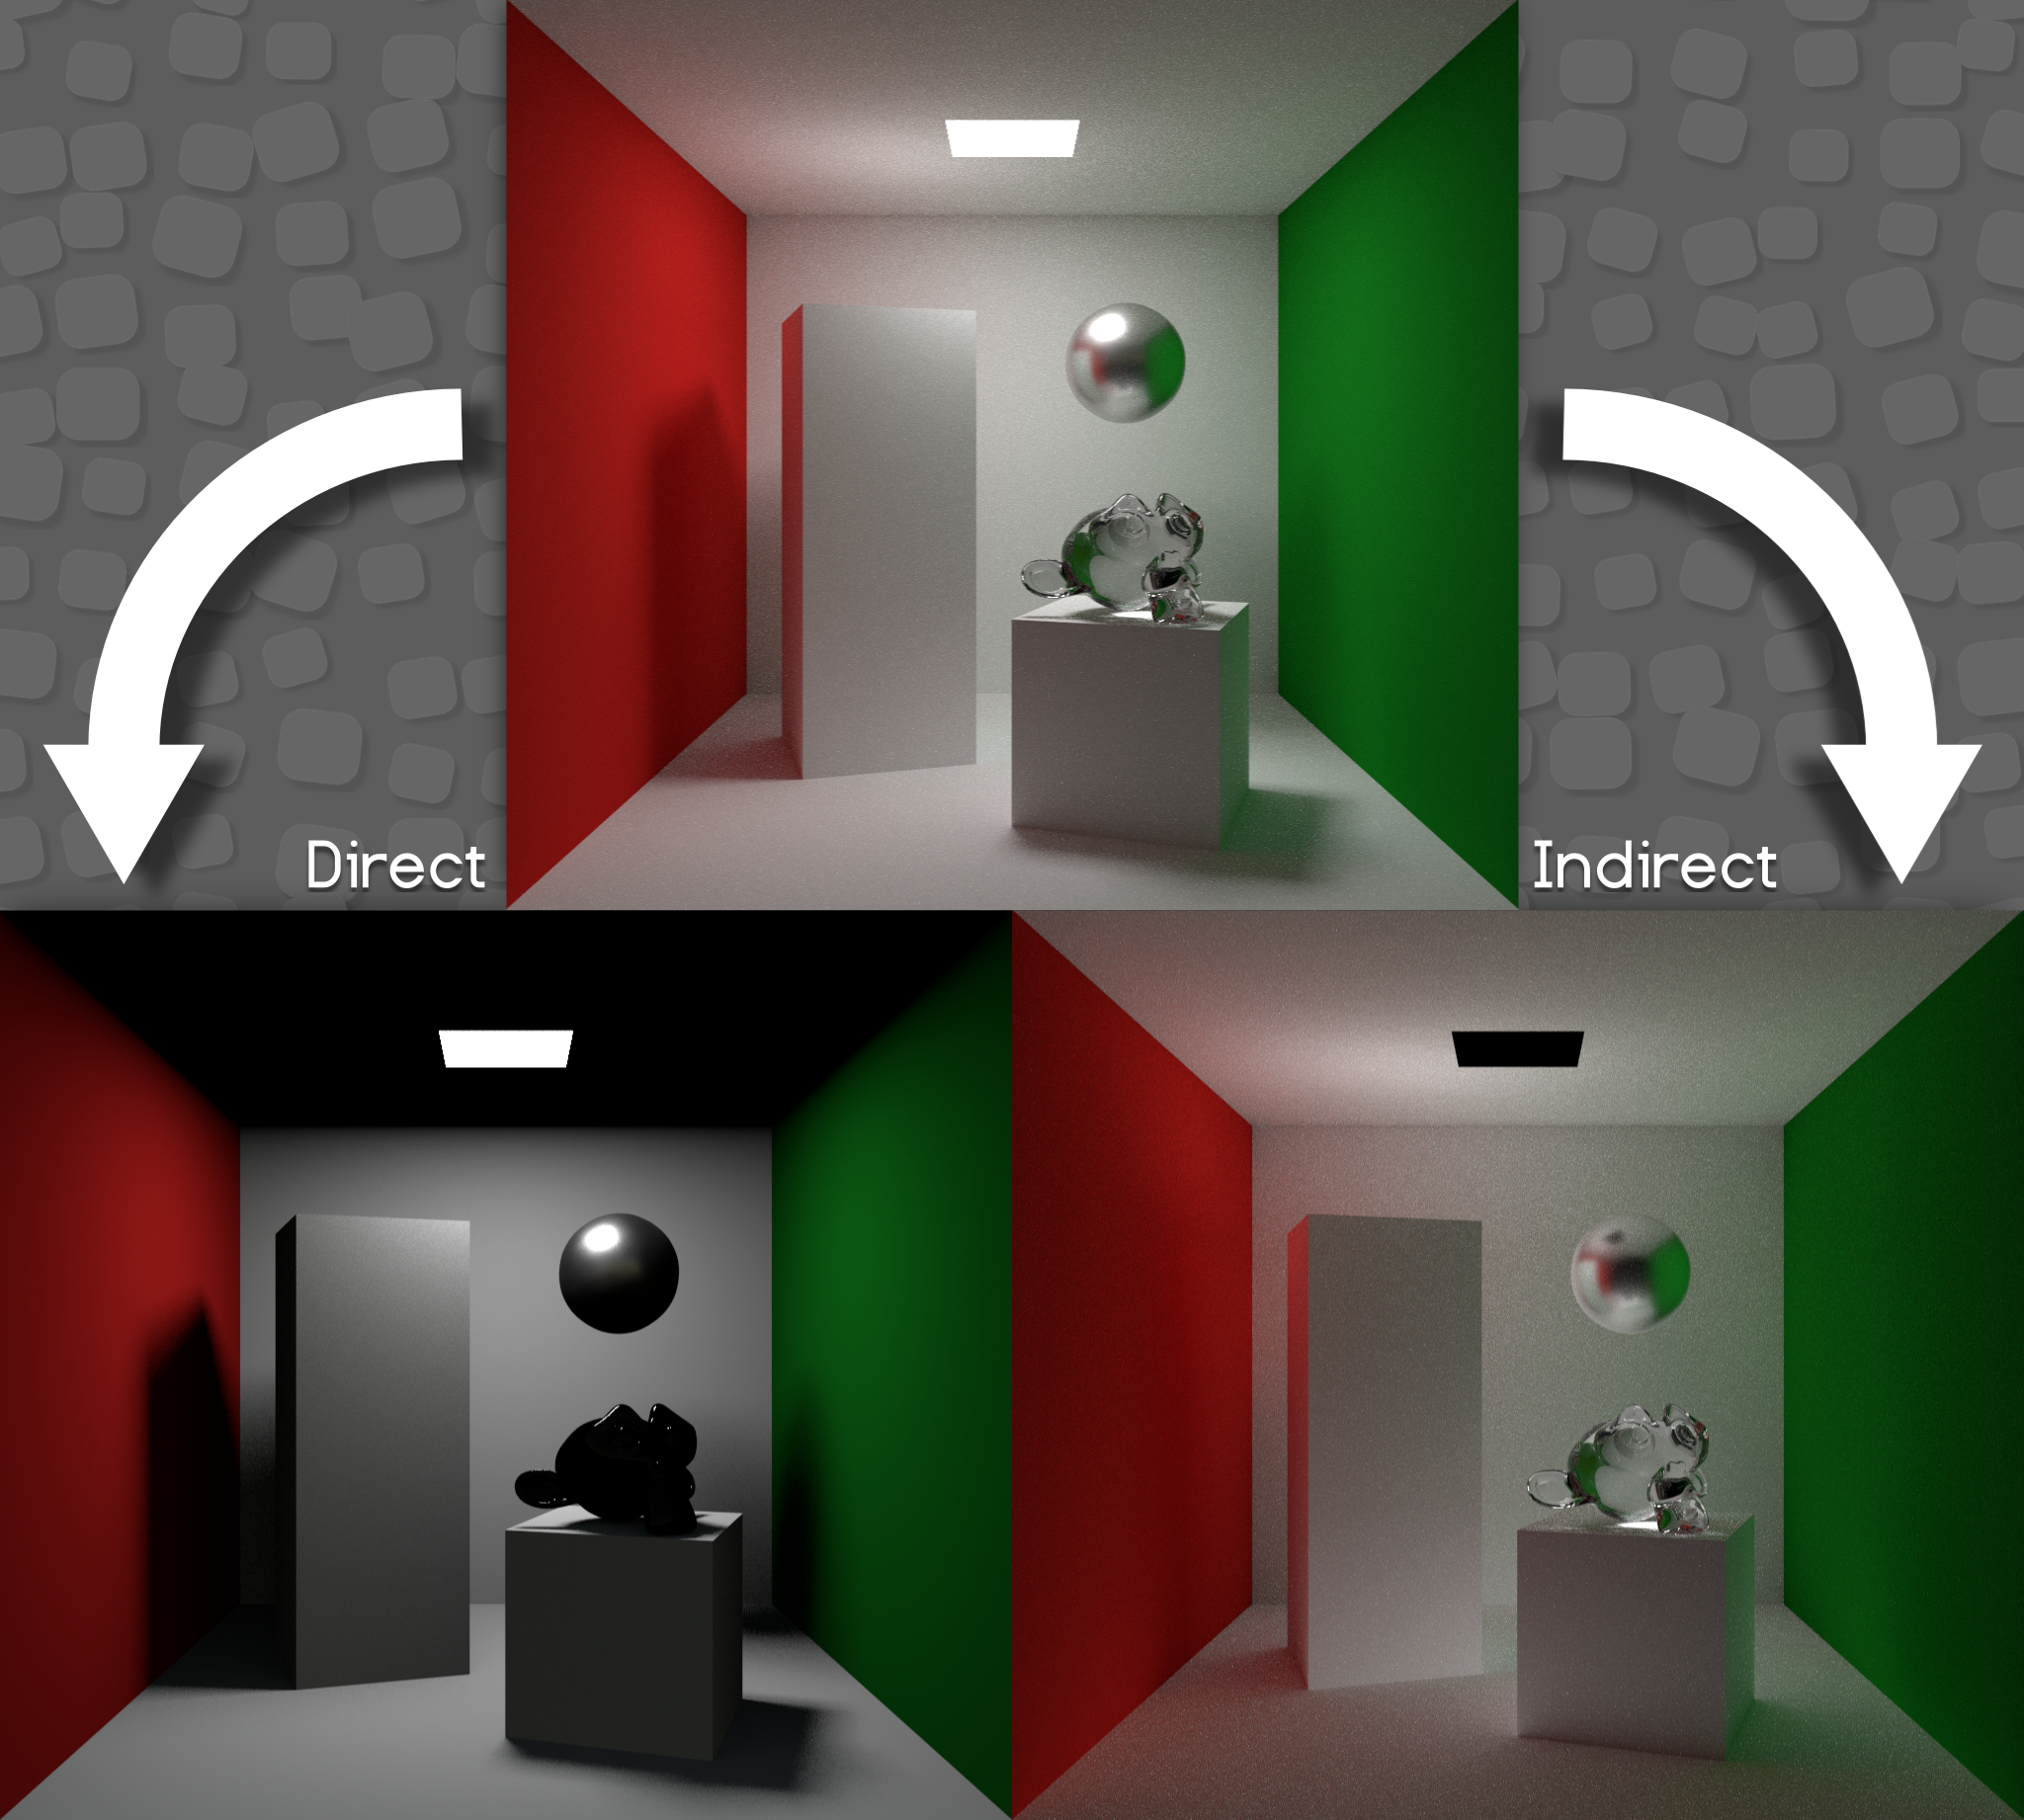
\includegraphics[width=\linewidth]{img/Lighting.png}
  \caption{Первичное и вторичное освещение 3D-сцены.}
  \label{fig:Lighting}
  \end{center}
\end{figure}

Современное программное обеспечение требует визуализации изображений с частотой кадров не менее 60 кадров в секунду с разрешением 1920x1600 пикселей и больше. Таким образом, временной бюджет на кадр составляет 16 миллисекунд. Соответственно, алгоритм вычисления глобального освещения должен выполняться за меньшее время для произвольной геометрии сцены. Отдельную сложность представляют приложения виртуальной реальности, так как в них стандартом считается 90 и 120 кадров в секунду при визуализации на 2 монитора с разрешением 4K (Рис. \ref{fig:VR}).

\begin{figure}[htb]
  \begin{center}
  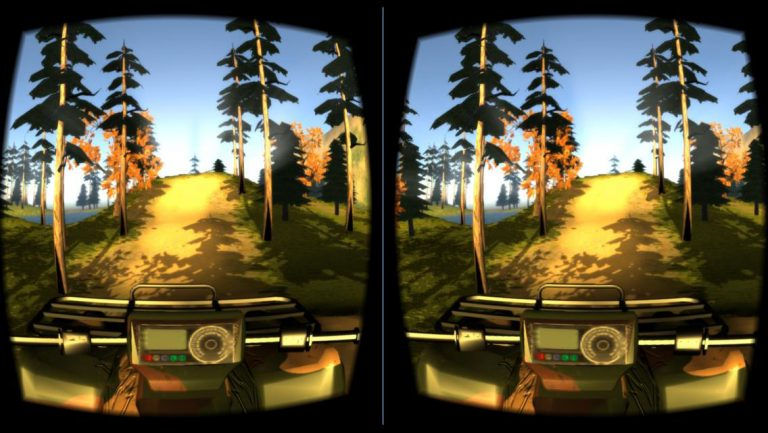
\includegraphics[width=\linewidth]{img/VR.jpeg}
  \caption{Пример экранов в приложении виртуальной реальности.}
  \label{fig:VR}
  \end{center}
\end{figure}

Отдельно выделяют диффузную компоненту освещения - свет, отраженные во всех направлениях и спекулярную (освещение, зависящее от позиции наблюдателя).

В данной работе предлагается модификация метода излучательности для вычисления диффузной компоненты вторичного освещения сцены. Вычислительная сложность классического метода излучательности квадратично зависит от количества элементов сцены. Так как в современных сценах количество элементов достигает миллионов, данный алгоритм применяют к упрощенным аналогам сцены \cite{Radiosity_simplification}. Но на больших сценах использование грубого приближения приводит к заметному ухудшению качества изображений.

В качестве решения предлагается использовать в вычислениях только геометрию вокруг наблюдателя, которая вносит наибольший вклад в изображение \cite{Anton}. Для этого необходимо добавлять элементы сцены в вычисления и исключать их при движении наблюдателя. Помимо этого предлагается использовать оптимизацию связанную с учётом нескольких отражений света внутри матрицы форм-факторов.

Использование матрицы форм-факторов нескольких отражений позволяет существенно сократить время вычисления \cite{Radiosity_multibounce}. Для этого был разработан метод пересчёта форм-факторов матрицы нескольких отражений при добавлении нового элемента сцены.

\sect{Формальная постановка задачи}

Исходные данные (составляют 3D-сцену либо её приближение):

\begin{enumerate}
	\item Patches - множество площадок в трехмерном пространстве. Для каждой площадки определены: 
	\begin{enumerate}
		\item положение - 4 точки в трехмерном пространстве, лежащие на одной плоскости.
		\item нормаль (вектор в 3D-пространстве);
		\item цвет, заданный в формате RGB (от 0 до 255);
		\item светимость --- 3-компонентный вектор в формате RGB32F (компоненты задаются 32-битными числами с плавающей точкой).
	\end{enumerate}
	\item Наблюдатель - камера, параметрами которой определяется проекция 3D-сцены на экран. Параметры камеры:
	\begin{enumerate}
		\item Позиция - вектор в 3D-пространстве.
		\item Направление.
		\item Разрешение камеры - размер итогового изображения в пикселях.
	\end{enumerate}
	\item События изменения в сцене:
	\begin{enumerate}
		\item Изменение светимости площадок.
		\item Изменение параметров камеры.
	\end{enumerate}
\end{enumerate}

События могут быть заданы программно или созданы в интерактивном режиме посредством устройств ввода.

Результатом работы алгоритма будет вектор 3-компонентных чисел, задающий глобальной освещение площадок в формате RGB.

Требуется:
\begin{enumerate}
	\item Вычислять глобальное освещение сцены для текущей конфигурации сцены с возможностью перемещения позиции камеры и изменения светимости квадов. 
	\item При этом время работы алгоритма не должно превышать 16 миллисекунд (для обеспечения N кадров в секунду). 
	\item Решение должно быть масштабируемым для произвольного размера сцены и современных разрешений экранов.
\end{enumerate}

\sect{Обзор существующих решений}

На данный момент существует ряд методов вычисления глобального освещения. Часть из них базируется на создании воксельной сетки, хранящей информацию об освещении, другие моделируют распространение света между поверхностями.

\subsect{Методы не требующие предобработки сцены}

Reflective Shadow Maps \cite{RSM} является одним из наиболее популярных методов интерактивного глобального освещения, и представляет собой вариацию метода Instant Radiosity \cite{InstantRadiosity} -- добавление в сцену вторичных источников света (Рис. \ref{fig:IR}). Основным недостатком является низкая точность получаемого решения, а преимуществом -- высокая скорость. Хотя подобные методы (называемые “many light”) активно развиваются \cite{ManyLight}, за исключением RSM они не часто применяются в интерактивных приложениях в силу не слишком хорошего баланса скорость/качество: в случае акцента на скорости, мы получаем RSM, а при стремлении к высокому качеству --- методы, слишком далекие от реального времени \cite{Lightcuts, LightSlice}.

\begin{figure}[htb]
  \begin{center}
  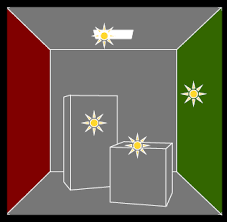
\includegraphics[width=0.5 \linewidth]{img/IR.png}
  \caption{Вторичные источники света в методе Instant Radiosity.}
  \label{fig:IR}
  \end{center}
\end{figure}

Voxel Cone Tracing \cite{VCT} использует пред-интегрированное освещение и сбор при помощи трассировки конусов. Метод обладает высокой точностью, однако же не лишён артефактов и является трудоемким в вычислительном плане. Для сцены создаётся несколько уровней воксельных сеток. Во время визуализации из каждого пикселя производится трассировка нескольких конусов (Рис. \ref{fig:VCT}). Чем дальше конус трассиуется от пикселя, тем более крупная воксельная сетка выбирается для трассировки. При достижении вокселя, содержащео геометрию в пиксель добавляется освещение данного вокселя.

На практике методом VCT как правило вычисляют только 1 отражение вторичного освещения ввиду высокой вычислительной сложности метода. Другим недостатком метода является отсутствие затенения от тонких стен на расстоянии. Это связано с использованием больших вокселей для приближения далёких частей сцены.

\begin{figure}[htb]
  \begin{center}
  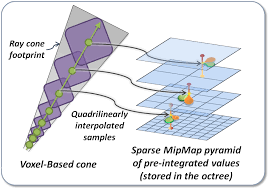
\includegraphics[width=0.5 \linewidth]{img/VCT.png}
  \caption{Трассировка конусом в методе Voxel Cone Tracing.}
  \label{fig:VCT}
  \end{center}
\end{figure}

Light Propagation Volumes \cite{LPV} численно решает дифференциальное уравнение уравнение на трехмерной сетке (Рис. \ref{fig:LPV}). Основными недостатком является низкая точность и высокие затраты памяти на регулярную сетку. Некоторые модификации метода используют разреженную сетку. Cascaded LPV \cite{CascadedLPV} амортизирует, но не решает всех проблем метода. Приближение геометрии воксельной сеткой приводит к "протечкам" света через геометрию сцены.

\begin{figure}[htb]
  \begin{center}
  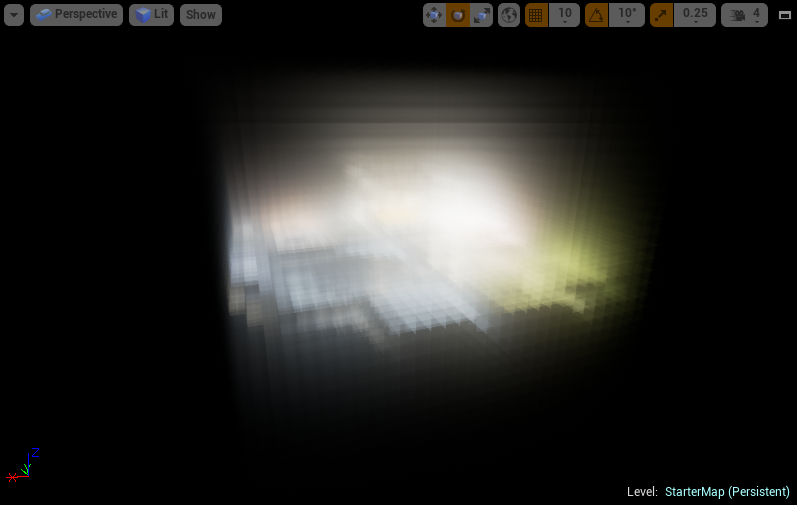
\includegraphics[width=0.8 \linewidth]{img/LPV.png}
  \caption{Трехмерная сетка в методе Light Propagate Volumes.}
  \label{fig:LPV}
  \end{center}
\end{figure}

\subsect{Методы требующие предобработки сцены}

Рассмотренные ранее методы решают задачу глобального освещения, пересчитывая освещение целиком каждый кадр. Они не могут достичь высокого качества при хорошей скорости т.к. глобальное освещение -- вычислительно трудоемкая задача по определению. С другой стороны, методы, использующие в том или ином виде предобработку могут добиться лучших результатов благодаря тому, что они выносят наиболее тяжёлые вычисления на этап предрасчета. Среди этих методов следует выделить 3 основных класса -- методы на основе сферических гармоник \cite{SPH}, излучательность \cite{RadiosityAndGI} и нейросетевые методы \cite{NNGI}.

Методов, использующих сферические гармоники в действительности достаточно много \cite{SPH, RadianceHints, PRT, ClusteredPRT, PRT2}. Их базовая идея исходит из Radiance Caching technique: компактное хранение падающей освещенности при помощи её разложения в базисе ортогональных функций (Рис. \ref{fig:SPH}). Далее, работая по аналогии с relighting \cite{RadianceHints, Relighting}, эти методы позволяют заменять окружение и пересчитывать освещение в динамике, складывая вклад от гармоник так же, как relighting складывает вклад от разных источников, суммируя отдельные изображения. Эти методы хорошо подходят для наружных сцен, но плохо применимы в интерьерных сценах поскольку гармоники считают что свет приходит в точку из бесконечно удаленных объектов. В интерьерах это правило нарушается, что приводит к различного вида артефактам --- от протечек до некорректного освещения \cite{RT_rendering}.

\begin{figure}[htb]
  \begin{center}
  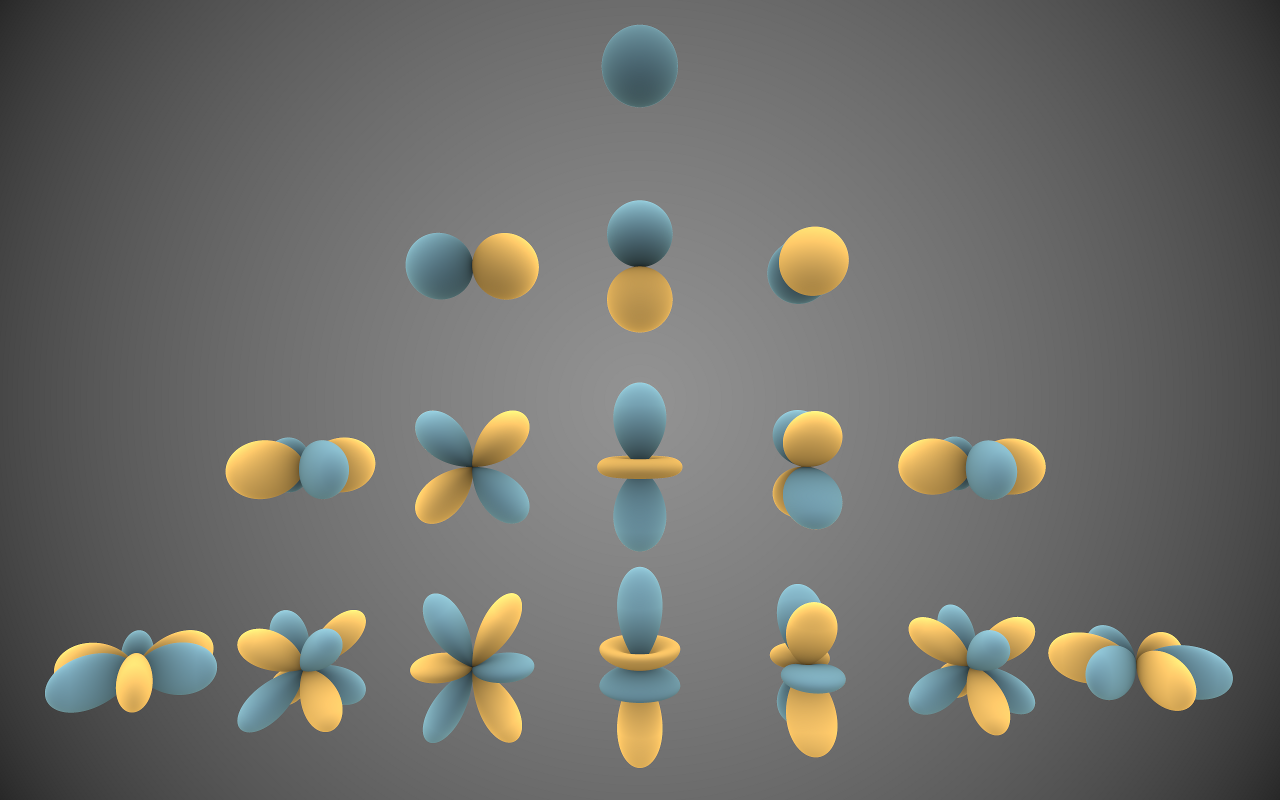
\includegraphics[width=0.95\linewidth]{img/SPH.png}
  \caption{Базисные функции в методе сферических гармоник.}
  \label{fig:SPH}
  \end{center}
\end{figure}

Вычисление глобального освещение на основе нейросетей является относительно новым направлением исследований и в работе \cite{NNGI} показывают высокую точность при реальном времени и компактном представлении в памяти (Рис. \ref{fig:NNGI}). К недостаткам метода следует отнести длительный предрасчет и полную статичность сцены -- геометрия и материалы не могут меняться (в методах на основе гармоник, например, эти ограничения, как правило, можно ослабить).

\begin{figure}[htb]
  \begin{center}
  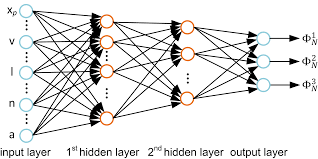
\includegraphics[width=0.5\linewidth]{img/NNGI.png}
  \caption{Архитектура нейронной сети, вычисляющей глобальное освещение.}
  \label{fig:NNGI}
  \end{center}
\end{figure}

\subsect{Метод излучательности}

Метод излучательности - физически корректная аппроксимация освещения \cite{RadiosityAndGI}. Метод широко используется в графических приложениях реального времени \cite{Enlighten} и светотехнике \cite{Dialux, Relux}.


Данный алгоритм позволяет свести вычисление глобального освещения к операциям умножения матрицы на вектор. Он делится на две стадии:
\begin{enumerate}
	\item Предобработка сцены.
	\item Вычисление освещения в реальном времени.
\end{enumerate}

Предобработка выполняется по следующему сценарию:
\begin{enumerate}
	\item Для сцены создаётся её упрощенный аналог исходной сцены (Рис. \ref{fig:Simplified}).
\begin{figure}[htb]
  \begin{center}
  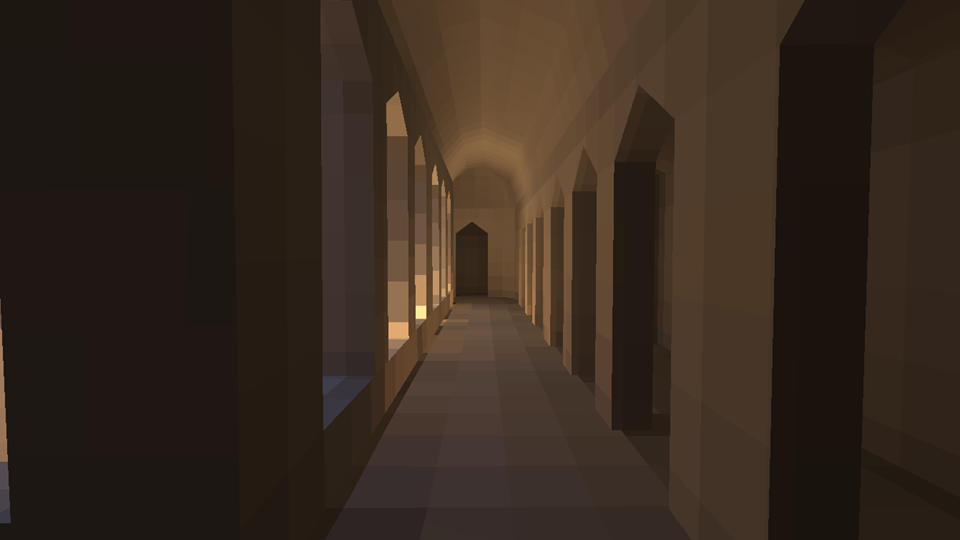
\includegraphics[width=\linewidth]{img/Simplified.png}
  \caption{Пример низкополигональной упрощенной сцены.}
  \label{fig:Simplified}
  \end{center}
\end{figure}
	
	\item Создаётся множество площадок(полигонов) сцены $patches$.
	\item Для каждой пары площадок вычисляются форм-факторы. Форм-фактор - число, показывающее, какая часть освещения перешла с одной площадки на другую. Форм-факторы вычисляются методом Монте-Карло. Для этого трассируются лучи между площадками и каждый луч, не встретивший препятствие, вносит свой вклад в форм-фактор.
	\item Из попарных форм-факторов формируется матрица $F$.
	\item Для площадок вычисляется их цвет как средний цвет элементов исходной сцены соответствующих площадке $Colors$.
	\item В случае использования матрицы нескольких отражений вычисляется полином матрицы форм-факторов $F_{multibounce}$.
\end{enumerate}

	Данные, полученные во время предобработки сцены, используются для вычисления глобального освещения в реальном времени:
\begin{enumerate}
	\item Вычисляется вектор изначальной светимости площадок. Он задаёт нулевое отражение света.
	\item Для $K$ отражений:
	\begin{enumerate}
		\item Матрица форм-факторов умножается на вектор предыдущего отражения света. Получается вектор $incident$ (\ref{eq:incident}).
		\begin{equation}
		incident_i = F \cdot excident_{i - 1}
		\label{eq:incident}
		\end{equation}
		\item Вектор $incident$ покомпонентно умножается на вектор цветов площадок. В результате получается вектор следующего отражения света (\ref{eq:excident}).
		\begin{equation}
		excident_i = incident_i \circ Colors
		\label{eq:excident}
		\end{equation}
	\end{enumerate}
	\item Векторы для всех отражений суммируются и получается вектор глобального освещения (\ref{eq:indirect}).
	\begin{equation}
	indirect = \sum\limits_{i = 1}^K incident_i
	\label{eq:indirect}
	\end{equation}
	\item Глобальное освещение используется при визуализации сцены.
\end{enumerate}

В данной работе за основу был выбран метод излучательности из-за её физической корректности, относительно высокой точности и скорости при малом числе площадок. Кроме того, этот метод один из самых простых в применении и хорошо ложиться на GPU, поскольку он может быть сведен к единичному умножению матрицы на вектор \cite{Radiosity_multibounce}. С другой стороны, недостатками метода излучательности являются: (1) зависимость по памяти и вычислениям как $O(N^2)$ от числа площадок и (2) статичность геометрии сцены (при этом, в отличие от метода на основе нейросетей, материалы могут быть легко заменены).

Данная работа направлена на устранение этих недостатков. Предложенный метод, таким образом, является в некотором смысле промежуточным звеном между методами, которые рассчитывают всё освещение каждый кадр и методами, полностью полагающимися на предрасчет.

\sect{Исследование и построение решения задачи}

В данном разделе описывается предложенный подход к вычислению глобального освещения методом излучательности для окрестности наблюдателя.

\subsect{Композиция форм-факторов}

Идея матрицы нескольких отражений базируется на композиции форм-факторов. Умножение матрицы форм-факторов самой на себя даёт матрицу, в которой учитывается переход света между площадками в ходе двух отражений (\ref{eq:compose}).
\begin{equation}
f_{second\ bounce(i, j, k)} = F_{ij} \cdot Colors_j \cdot F_{jk}
\label{eq:compose}
\end{equation}

Соответственно, результатом умножения матрицы, форм-факторов на вектор форм-факторов, будет вектор форм-факторов для двух отражений света (\ref{eq:compose_column}).
\begin{equation}
f_{second\ bounce(i)} = F \cdot (Colors \circ F_i)
\label{eq:compose_column}
\end{equation}

Таким образом, можно получить вектор форм-факторов для произвольных конфигураций отражений.

\subsect{Обновление матрицы форм-факторов}

Использование локальной матрицы позволяет значительно сократить количество вычислений. Но в то же время, каждое изменение положения наблюдателя, приводит к изменению локальной матрицы. Из неё необходимо удалить информацию о лишних площадках и добавить информацию о площадках, которые появились в окрестности камеры.

\subsect{Удаление площадки}

Удаление площадки из матрицы форм-факторов реализуется очищением соответствующих строк и столбца. 

\subsect{Добавление площадки}

Операция добавления площадки в матрицу форм-факторов осуществляется в несколько этапов:
\begin{enumerate}
	\item Вначале учитываются форм-факторы из обычной матрицы. $F_{row}$ - строка форм-факторов, $F_{column}$ - вектор-столбец форм-факторов.
	\item Вычисляется форм-фактор для двойного отражения новой площадки:
	\begin{equation}
	double\_reflection = F_{column} \cdot (Colors \circ F_{row})
	\label{eq:double_reflection}
	\end{equation}
	\item Вычисление форм-факторов для тройного отражения.
	\begin{enumerate}
		\item Вначале вычисляется отражение только между новой площадкой и остальными площадками в матрице: 
		\begin{equation}
		G_{columng} = F_{column} \cdot color_{new} * double\_reflection
		\end{equation}
		\begin{equation}
		G_{row} = F_{row} \cdot color_{new} * double\_reflection
		\end{equation}
		\item Затем вычисляется тройное отражение с учетом переотражений внутри матрицы: 
		\begin{equation}
		G_{column}' = localMatrix \cdot G_{column}
		\end{equation}
		\begin{equation}
		G_{row}' = G_{row} \cdot localMatrix
		\end{equation}
	\end{enumerate}
	\item Обновление остальных значений матрицы:
	\begin{equation}
	localMatrix = localMatrix + G_{row} \cdot G_{column}
	\end{equation}
\end{enumerate}

\subsect{Вычисление освещения}

Для матрицы нескольких отражений вычисление освещения сводится к единственному умножению матрицы на вектор. Исходя из этого, достаточно вычислить освещение только для видимых площадок. Матрица нескольких отражений может использоваться с умножением только площадок с ненулевой начальной светимостью.
Таким образом, вычисление освещения выполняется операцией умножения матрицы размера $M_{visible} \times M_{emitted}$ на вектор размера $M_{emitted}$.

\sect{Описание практической части}

В ходе работы была разработана программная реализация алгоритма на языках C++ и GLSL.

Для вычислений на видеокарте была использована библиотека OpenGL версии 4.6.

Объем кода для CPU: 7486 строк.

Объем кода для GPU: 676 строк.

Реализовано 8 вычислительных ядер на основе технологии Compute Shaders в OpenGL.

Тестирование проводилось на сцене содержащей 63125 площадок.

Библиотека OpenGL была выбрана ввиду её кросплатформенности. Реализация способна работать на ОС семейств Windows и Unix. В частности проводились запуски на Windows 10 и Ubuntu 18.04.

\subsect{Сравнение изображений}

В ходе работы было проведено сравнение изображений с обычным методом излучательности и методом трассировки путей.

\begin{figure}[htb]
  \begin{center}
  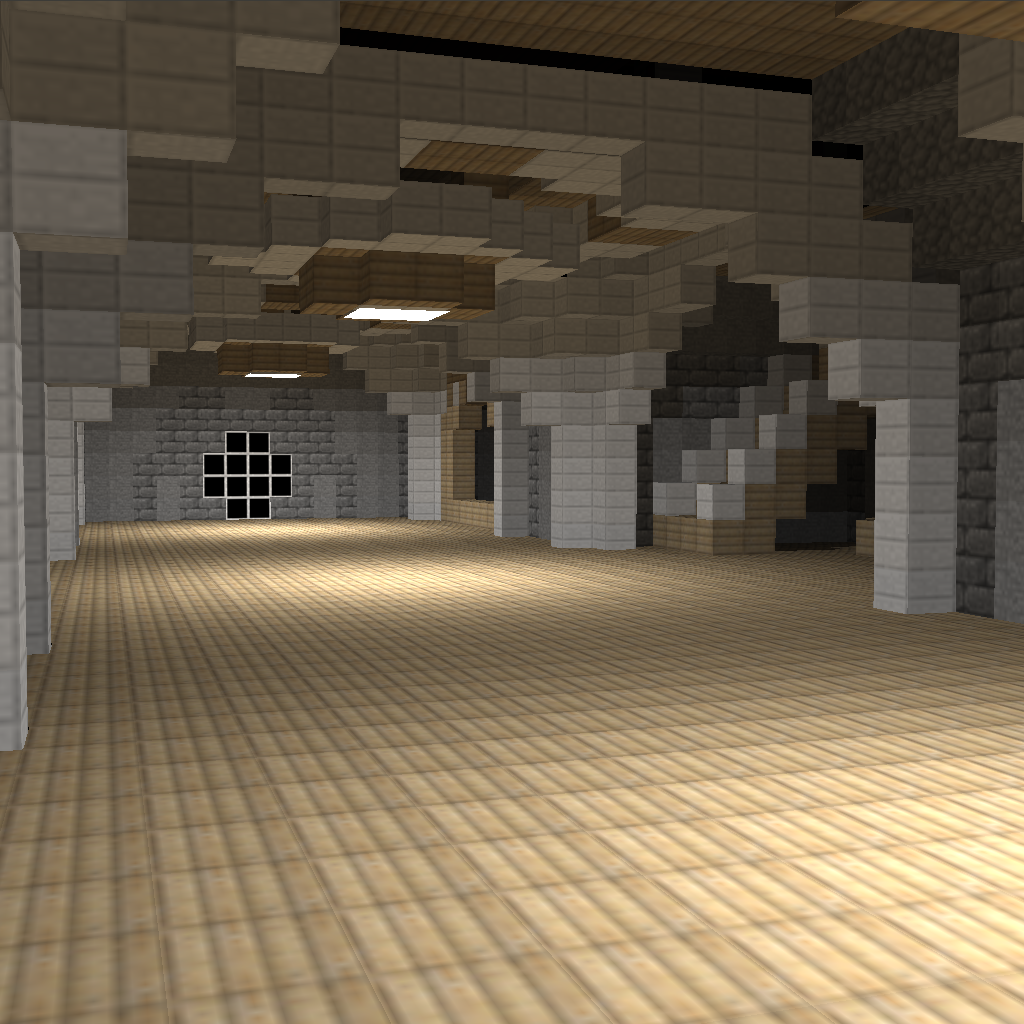
\includegraphics[width=0.32\linewidth]{img/DynamicRadiosity1.png}
  \includegraphics[width=0.32\linewidth]{img/PathTracing1.png}
  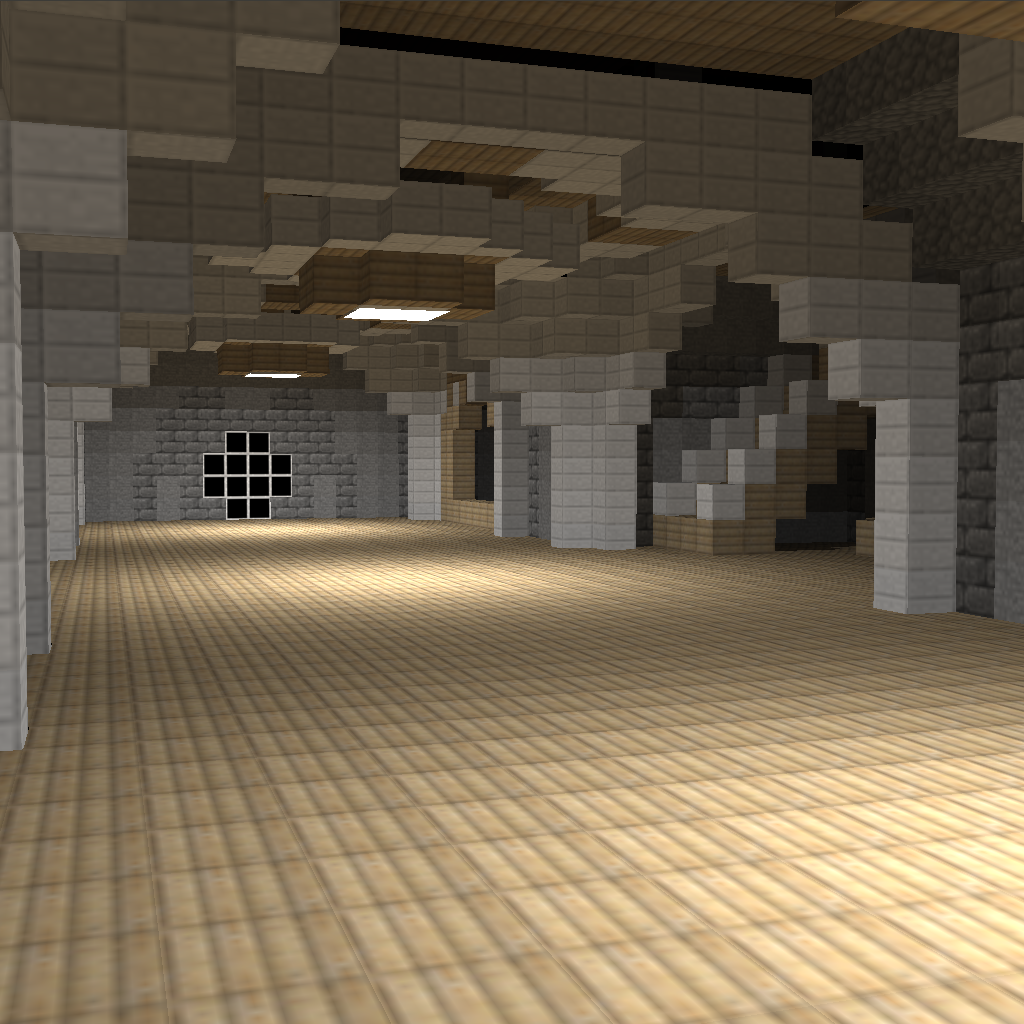
\includegraphics[width=0.32\linewidth]{img/Radiosity1.png}
  \caption{Сравнение изображений: (1) Предложенный метод, (2) Метод трассировки путей, (3) Метод излучательности}
  \label{fig:ImageComparison1}
  \end{center}
\end{figure}

\begin{figure}[htb]
  \begin{center}
  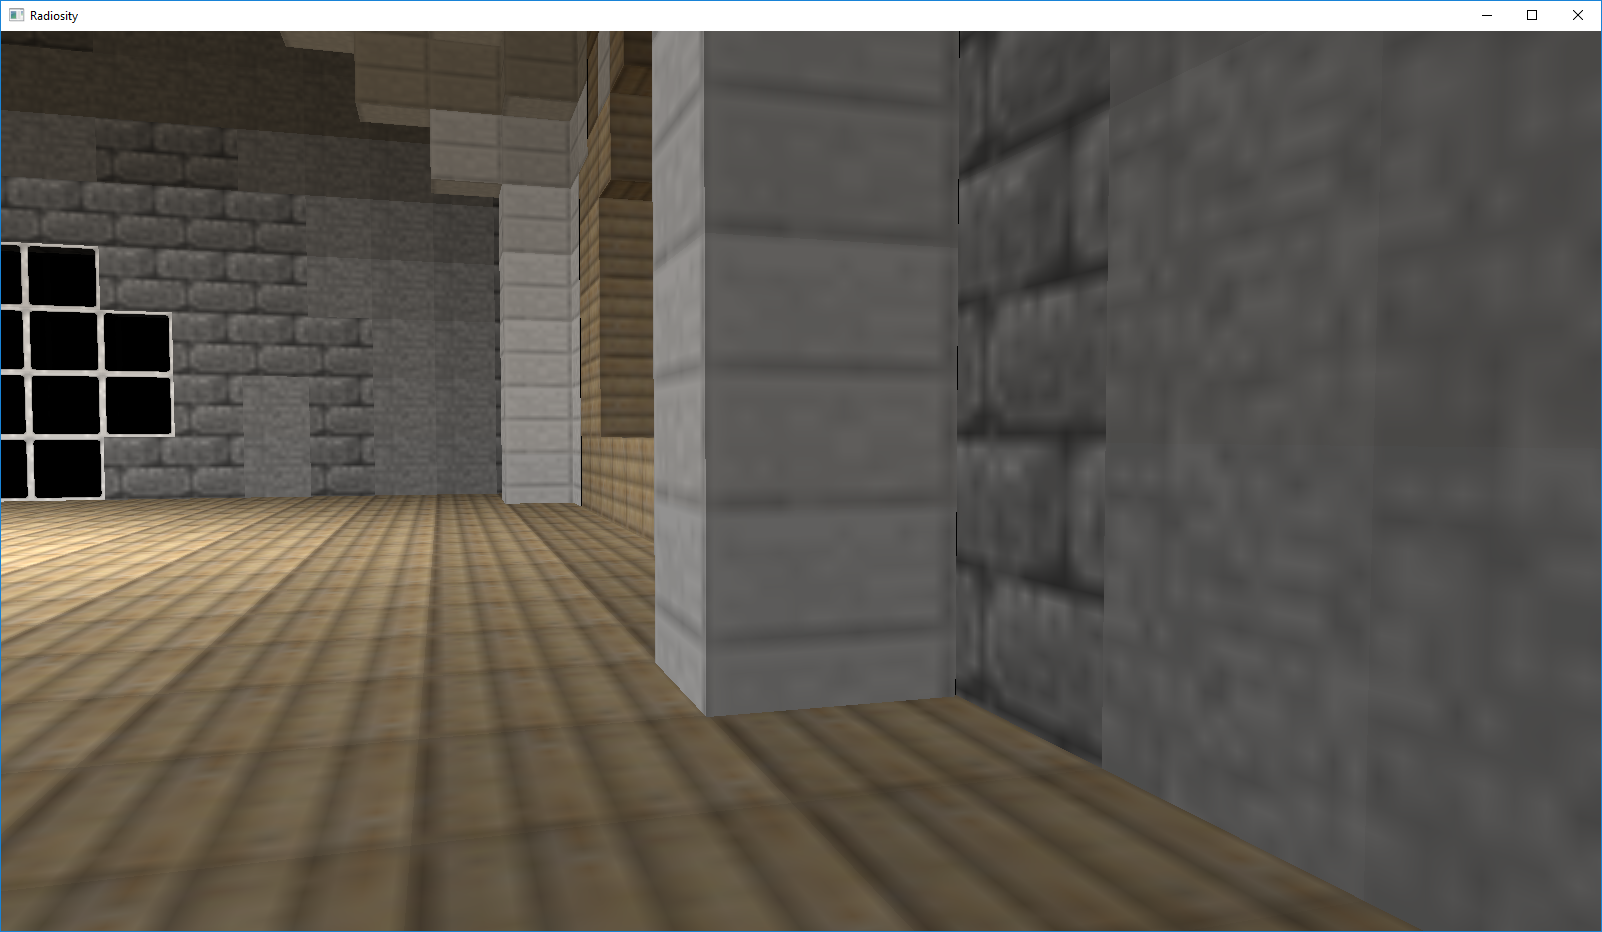
\includegraphics[width=0.48\linewidth]{img/ADynamic_radiosity.png}
  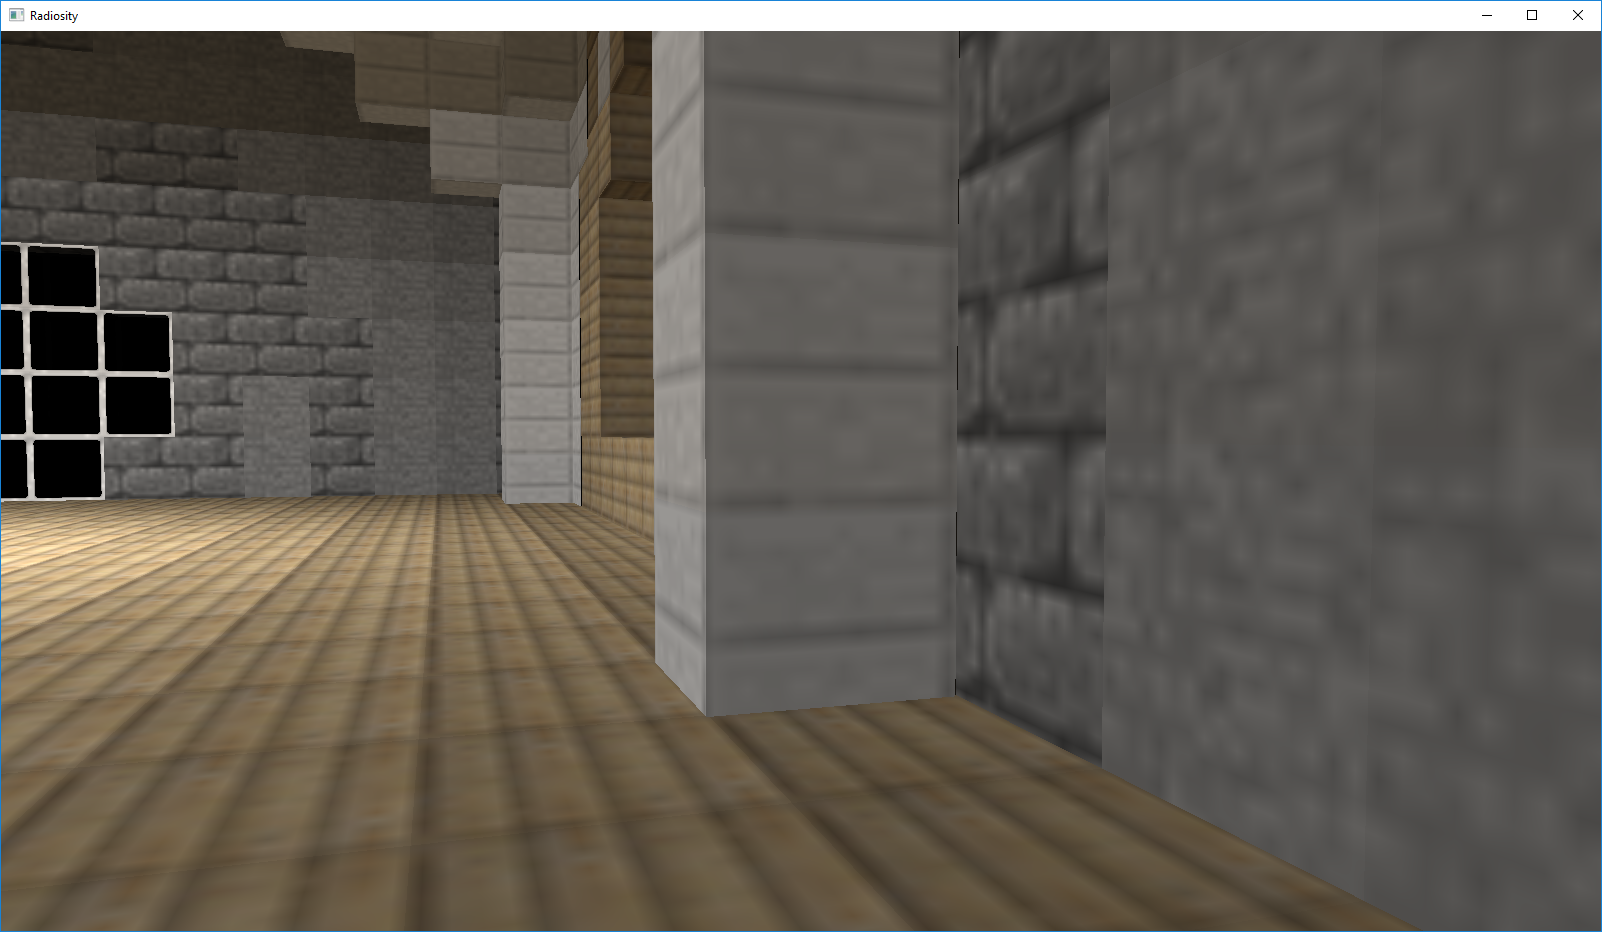
\includegraphics[width=0.48\linewidth]{img/ARadiosity.png}
  \caption{Сравнение изображений: (1) Предложенный метод, (2) Метод излучательности}
  \label{fig:ImageComparison2}
  \end{center}
\end{figure}

Освещение на дальних площадках соответсвуют методу излучательности при неизменном освещении. Для ближних патчей освещение различается незначительно.

\subsect{Сравнение времени работы}

\begin{figure}[htb]
  \begin{center}
  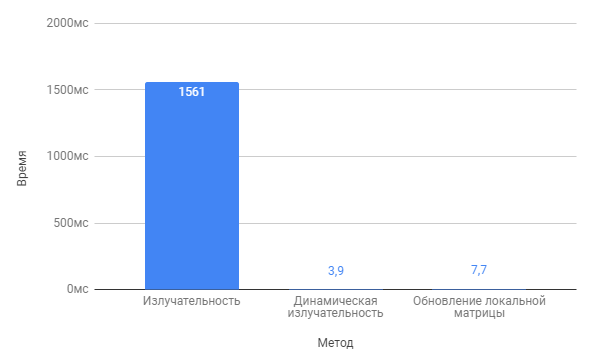
\includegraphics[width=0.7\linewidth]{img/Timings.png}
  \caption{Сравнение времени работы методов}
  \label{fig:Timings}
  \end{center}
\end{figure}

Предложенный метод позволяет значительно ускорить вычисление глобального освещения за счёт сокращения области пересчёта.

\newpage

\sect{Заключение}

В ходе работы был разработан новый метод вычисления глобального освещения  вокруг наблюдателя, основанный на алгоритме излучательности.
Предложенный алгоритм имеет возможность изменять соотношение сложности вычисления и качества и существенно превосходит в этом исходный алгоритм излучательности.
На тестовой сцене время работы предложенного алгоритма в сотни раз меньше.



\begin{thebibliography}{00}

\bibitem{RT_rendering} Akenine-Möller T., Haines E., Hoffman N., Pesce A., Iwanicki M., Hillaire S. Real-Time Rendering, 4th edition. Boca Raton: Taylor \& Francis, 2018. 1199 p.

\bibitem{Radiosity_simplification} Щербаков А., Фролов В. Автоматическое упрощение геометрии для расчёта вторичной освещенности методом излучательности // Сборник трудов Графикон 2016. — ННГАСУ, 2016. — С. 34 –- 38.

\bibitem{Anton} Yudintsev A. Scalable Real-time Global Illumination for Large Scenes [PDF] (https://gdcvault.com/play/1026469/Scalable-Real-Time-Global-Illumination)

\bibitem{Radiosity_multibounce} Shcherbakov A., Frolov V. Accelerating radiosity on GPUs // WSCG'2017 Full papers proceedings. Computer Science Research Notes 2701 Pilsen, Czech Republic, 2017. P. 99 –- 105.

\bibitem{RSM} Dachsbacher C., Stamminger M. Reflective shadow maps // Proceedings of the 2005 symposium on Interactive 3D graphics and games. ACM, 2005. P. 203 -- 231.

\bibitem{InstantRadiosity} Keller A. Instant radiosity // In Proceedings of the 24th annual conference on Computer graphics and interactive techniques (SIGGRAPH '97). ACM Press/Addison-Wesley Publishing Co., New York, NY, USA, 1997. P. 49 -- 56. 

\bibitem{ManyLight} Dachsbacher C., Krivanek J., Hasan M., Arbree A., Walter B., Novak J. Scalable Realistic Rendering with Many-Light Methods // Computer Graphics Forum. 33. 2014. P. 88 -- 104.

\bibitem{Lightcuts} Walter, B., Fernandez, S., Arbree, A., Bala, K., Donikian, M., and Greenberg, D. P. Lightcuts: a scalable approach to illumination // In ACM Transactions on graphics (TOG) [N 3]. ACM, 2005. P. 1098 -- 1107

\bibitem{LightSlice} Ou, J., and Pellacini, F. LightSlice: matrix slice sampling for the many-lights problem // ACM Transactions on Computer Systems, 2011. P. 179:1 -- 179:8.

\bibitem{VCT} Crassin, C., Neyret, F., Sainz, M., Green, S., and Eisemann, E. Interactive indirect illumination using voxel cone tracing // In Computer Graphics Forum [N. 7], Oxford, UK: Blackwell Publishing Ltd, 2011. P. 1921 -- 1930.

\bibitem{LPV} Kaplanyan A. Light propagation volumes in CryEngine 3 // ACM SIGGRAPH Courses, 2009. P. 2.

\bibitem{CascadedLPV} Kaplanyan A., Dachsbacher C. Cascaded light propagation volumes for real-time indirect illumination // Proceedings of the 2010 ACM SIGGRAPH symposium on Interactive 3D Graphics and Games. ACM, 2010. P. 99 -- 107.

\bibitem{SPH} Green R. Spherical harmonic lighting: The gritty detail // Archives of the Game Developers Conference, 2003. P. 4.

\bibitem{RadiosityAndGI} Sillion F. X. et al. Radiosity and global illumination // San Francisco : Morgan Kaufmann, 1994. 251 p.

\bibitem{NNGI} Ren P., Wang J., Gong M., Lin S., Tong X., Guo B. Global illumination with radiance regression functions // ACM Transactions on Graphics (TOG), 2013. N 32. P. 12.

\bibitem{RadianceHints} Papaioannou G. Real-time diffuse global illumination using radiance hints //Proceedings of the ACM SIGGRAPH Symposium on High Performance Graphics. ACM, 2011. P. 15 -- 24.

\bibitem{PRT} Sloan P.-P., Kautz J., Snyder J. Precomputed radiance transfer for real-time rendering in dynamic, low-frequency lighting environments. ACM, 2002. P. 527 -- 536.

\bibitem{ClusteredPRT} Sloan P.-P., Hall J., Hart J., Snyder J. Clustered principal components for precomputed radiance transfer. ACM Trans. Graph., 2003. P. 382 -- 391.

\bibitem{PRT2} Kautz J., Lehtinen J., Sloan P.-P. SIGGRAPH Precomputed Radiance Transfer: Theory and Practice course. [HTML] (http://www0.cs.ucl.ac.uk/staff/J.Kautz/PRTCourse/)

\bibitem{Relighting} Dorsey J., Arvo J., Greenberg D. Interactive design of complex time dependent lighting // IEEE Computer Graphics and Applications. 1995. N. 15(2). P. 26 -- 36.

\bibitem{Enlighten} Martin S.  Enlighten real-time radiosity // ACM SIGGRAPH 2011 Computer Animation Festival. 2011. P. 97 -- 97.

\bibitem{Dialux} Mangkuto, R. A. Validation of DIALux 4.12 and DIALux evo 4.1 against the Analytical Test Cases of CIE 171 // Leukos. 2006. N. 12(3). P. 139 -- 150.

\bibitem{Relux} Yu X., Su Y., Chen X. Application of RELUX simulation to investigate energy saving potential from daylighting in a new educational building in UK // Energy and Buildings. 2014. N. 74. P. 191 -- 202.

\end{thebibliography}
\addcontentsline{toc}{chapter}{Список литературы}

\end{document}
